

\section{Problem 2}
\label{part2}
\begin{verbatim}
Gender homophily in your Twitter graph (5 points)

Take the Twitter graph you generated in question #1 and test for
male-female homophily.  For the purposes of this question you can
consider the graph as undirected (i.e., no distinction between
``follows'' and ``following'').  Use the twitter name (not ``screen
name''; for example ``Michael L. Nelson'' and not ``@phonedude_mln'')
and programatically determine if the user is male or female.  Some
sites that might be useful:

https://genderize.io/
https://pypi.python.org/pypi/gender-detector/0.0.4

Create a table of Twitter users and their likely gender.  List any 
accounts that can't be determined and remove them from the graph.

Perform the homophily test as described in slides 11-15, Week 7.

Does your Twitter graph exhibit gender homophily?

\end{verbatim}

\subsection{Solution}
\begin{enumerate}
\item This question is continuation of the above question with some changes. Here we need to use the output of the previous question and modify the output.
\item I need to find out the genders of all my followers and find out whether there is gender homophily or not.
\item I used follower's first name to find out their genders using the reference provided in the question.
\item So, I took all my followers list in json file and gave it as input to my python code which processes each follower's first name and gives their gender as output.
\item The python code used here can be found in listing\ref{lst:q2-1} and the sample output of it can be seen in figure\ref{Sample_t1}.
\item Then I created a new json file which includes all the follower's names,genders and I gave sample id for each of them. This can be seen here in figure\ref{Sample_t2}.
\item The output tells me whether a follower is ``Male'',``Female'' or ``Null''.
\item I removed all the users who have their gender as ``Null'' because it was said so in the question and this helps me to find gender homophily easily.
\item This json file is given as input to my html code which gives a force directed graph. The code of the html file can be seen in listing\ref{lst:q2-2}.
\item The working model of this d3 graph can be seen at this link \url{http://bl.ocks.org/PaladhiDinesh/c7ad7ffc4fb17f4f9411} and the sample screenshot of it can be seen in figure\ref{graph2}.
\item This is an undirected graph and when hovered on a node with the mouse pointer you can see the name of the follower. The nodes in blue are Male and in orange are Female.
\item This twitter graph exhibits gender homophily as we can easily see that more blue are more connected to blue nodes which says that Male followers are more connected to other Male followers.

\end{enumerate}

\begin{table}

\caption{Table with followers and gender}
\label{Table:q1table1}
\begin{center}
\begin{tabular}{| c | c |}
\hline

 Name | Gender\\ \hline
 erika  | female\\ \hline		
 varun  | male\\ \hline		
 Naina  | female\\ \hline		
 vamshi | male\\ \hline		
 Ravi  | male\\ \hline
 Shivani  | female\\ \hline	
 BhavaniManthena    | null\\ \hline
 manoj | male\\ \hline
 Rithika  | null\\ \hline	
 majetisiri| null\\ \hline
 Manish  | male\\ \hline	
 Kumaraswamy | male\\ \hline
 Prashanth  | male\\ \hline	
 Uday  | male\\ \hline
 Rithvik | null\\ \hline
 ashwin | male\\ \hline	
 TCAT | null\\ \hline
 NaveenKumar   | null\\ \hline	
 pravallika | null\\ \hline
 maithri  | null\\ \hline	
 KlaraAdrinson  | null\\ \hline
 DeonneLivingsto  | null\\ \hline
 LatrinaMcRattig  | null\\ \hline
MommyOddenino| 		null\\ \hline		
Nikilesh|	null\\ \hline		
Dinesh| 	male\\ \hline		
Joseph|	male\\ \hline		
Mohan| 		male\\ \hline
Vasavi|		female\\ \hline	
vineeth| 	male\\ \hline
harish`| 	male\\ \hline
pranay| 		null\\ \hline	
Sandeep| 		male\\ \hline
vani| 		female\\ \hline	
madhukar| 	male\\ \hline
Harish| 		male\\ \hline	
bharath|		male\\ \hline
sunny| 		male\\ \hline
Rajitha| 	female\\ \hline
bhanu	|	male\\ \hline		
mrut		|		null\\ \hline		
Akkineni				|	male\\ \hline		
Vaishampayan|			null\\ \hline		
Apoorva|	female\\ \hline
paladhi			|	null\\ \hline	
aruna| 		female\\ \hline
telugupopular| 		null\\ \hline
satvikgadam		|		null\\ \hline	
sudha		|		female\\ \hline
Sandeep   |  	male\\ \hline	
Ramya   |  	female\\ \hline	
    
\end{tabular}
\end{center}
\end{table}
\newpage

\subsection{Code Listing}

\lstinputlisting[language=Python,breaklines = true,frame=single,caption={Python Code for getting finding gender of each follower}, label=lst:q2-1,captionpos=b,numbers=left,showspaces=false,showstringspaces=false,basicstyle=\footnotesize]{get_gender.py}
\newpage

\subsection{Code Listing}

\lstinputlisting[language=Html,breaklines = true,frame=single,caption={HTML code with d3 to get force directed graph showing gender homophily}, label=lst:q2-2,captionpos=b,numbers=left,showspaces=false,showstringspaces=false,basicstyle=\footnotesize]{follower_gender.html}
\newpage

\subsection{Results}

\begin{figure}[ht]    
    \begin{center}
        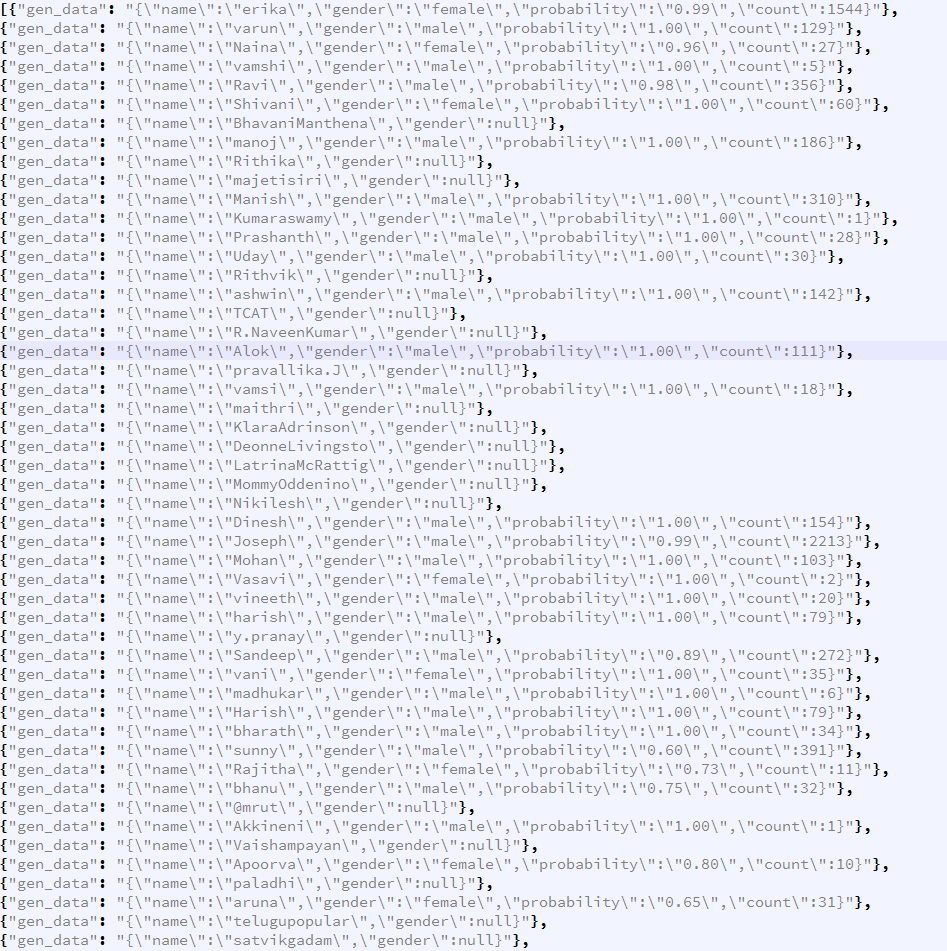
\includegraphics[scale=0.7]{sampe_gen_data.png}
        \caption{Sample list of generated genders for each follower}
        \label{Sample_t1}
    \end{center}
\end{figure}
\newpage
\subsubsection{Final json}
\begin{figure}[ht]    
    \begin{center}
        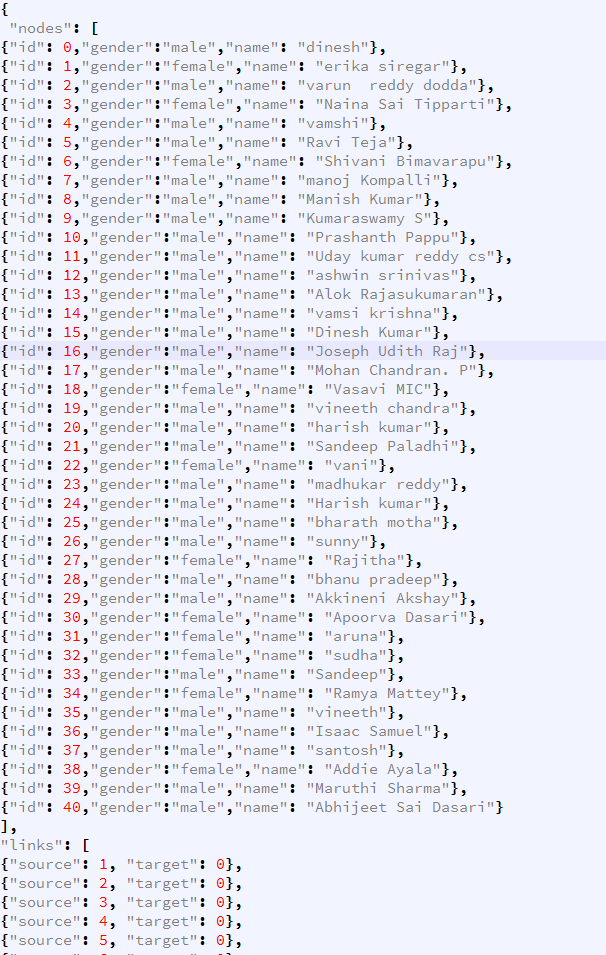
\includegraphics[scale=0.6]{sample_gender_json.png}
        \caption{Sample final json file with nodes as followers and links as friendship between them along with their gender}
        \label{Sample_t2}
    \end{center}
\end{figure}
\newpage

\subsubsection{D3 Graph}
\begin{figure}[ht]    
    \begin{center}
        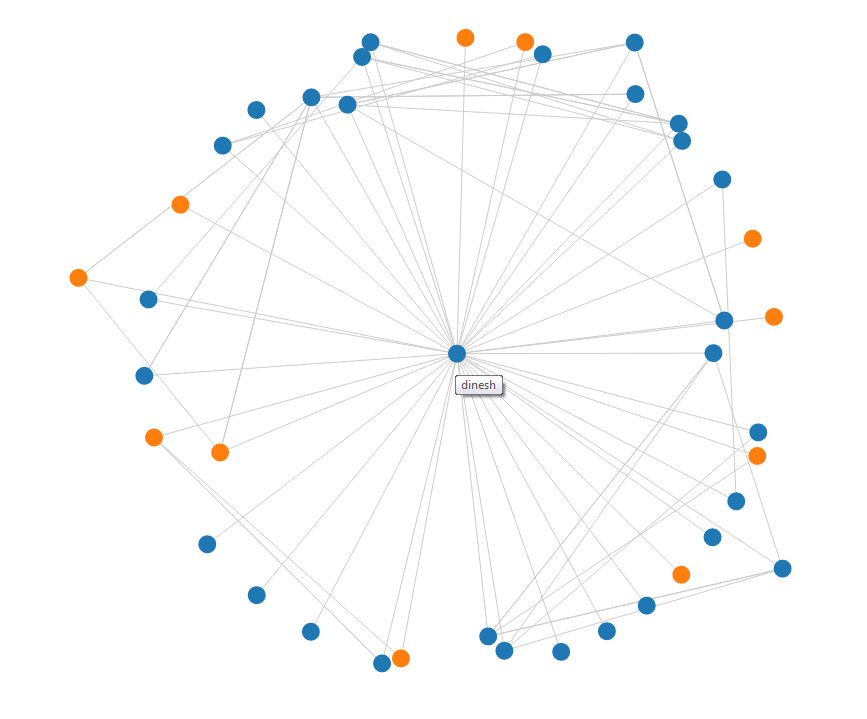
\includegraphics[scale=0.8]{gender_homophily.png}
        \caption{D3 Graph with gender homophily showing blue color nodes as ``Men'' and orange color nodes as ``Female'' }
        \label{graph2}
    \end{center}
\end{figure}
\newpage
